% ---------------------------------------------------------------------------
% ---------------------------------------------------------------------------
% Modelo LaTex para preparação do documento final de Dissertação de Mestrado
% O modelo está em conformidade com ABNT NBR 14724:2011: 
% Programa de Pós-Graduação em Informática
% Universidade Federal de Alagoas
% Versão: v0.9
% ---------------------------------------------------------------------------
% ---------------------------------------------------------------------------

\PassOptionsToPackage{inline}{enumitem}

\documentclass[
	% -- opções da classe memoir --
	12pt,					% tamanho da fonte
	openright,				% capítulos começam em páginas ímpares (insere página vazia caso preciso)
	twoside,				% para impressão em verso e anverso. Oposto a oneside
	a4paper,				% tamanho do papel. 
	% -- opções da classe abntex2 --
	chapter=TITLE,			% títulos de capítulos convertidos em letras maiúsculas
	%section=TITLE,			% títulos de seções convertidos em letras maiúsculas
	%subsection=TITLE,		% títulos de subseções convertidos em letras maiúsculas
	%subsubsection=TITLE,	% títulos de subsubseções convertidos em letras maiúsculas
	% -- opções do pacote babel --
	english,				% idioma adicional para hifenização
	%french,				% idioma adicional para hifenização
	%spanish,				% idioma adicional para hifenização
	brazil					% o último idioma é o principal do documento
]{abntex2}

% ---------------------
% Pacotes OBRIGATÓRIOS
% ---------------------
\usepackage[T1]{fontenc}		% Seleção de códigos de fonte.
\usepackage[utf8]{inputenc}		% Codificação do documento (conversão automática dos acentos)
\usepackage{lastpage}			% Usado pela Ficha catalográfica
\usepackage{indentfirst}		% Identa o primeiro parágrafo de cada seção.
\usepackage{color}				% Controle das cores
\usepackage{graphicx,graphicx}	% Inclusão de gráficos
\usepackage{epsfig,subfig}		% Inclusão de figuras
\usepackage{microtype} 			% Melhorias de justificação
% ---------------------
		
% ---------------------
% Pacotes ADICIONAIS
% ---------------------
\usepackage{lipsum}						% Geração de dummy text
\usepackage{amsmath,amssymb,mathrsfs}	% Comandos matemáticos avançados 
\usepackage{setspace}  					% Para permitir espaçamento simples, 1 1/2 e duplo
\usepackage{verbatim}					% Para poder usar o ambiente "comment"
\usepackage{tabularx} 					% Para poder ter tabelas com colunas de largura auto-ajustável
\usepackage{afterpage} 					% Para executar um comando depois do fim da página corrente
\usepackage{url} 						% Para formatar URLs (endereços da Web)
\usepackage{svg}
% ---------------------

% ---------------------
% Pacotes de CITAÇÕES
% ---------------------
\usepackage[brazilian,hyperpageref]{backref}  % Paginas com as citações na bibliografia
\usepackage[alf]{abntex2cite}				  % Citações padrão ABNT (alfa)
%\usepackage[num]{abntex2cite}				  % Citações padrão ABNT (numéricas)
% ---------------------

% Definição de diretório de imagens
\graphicspath{{imagens/}}

% Configurações de CITAÇÕES para abntex2
% --- 
% CONFIGURAÇÕES DE PACOTES
% --- 

% ---
% Configurações do pacote backref
% Usado sem a opção hyperpageref de backref
\renewcommand{\backrefpagesname}{Citado na~(s) página~(s):~}
% Texto padrão antes do número das páginas
\renewcommand{\backref}{}
% Define os textos da citação
\renewcommand*{\backrefalt}[4]{
	\ifcase #1 %
		Nenhuma citação no texto.%
	\or
		Citado na página #2.%
	\else
		Citado #1 vezes nas páginas #2.%
	\fi}%
% ---

% Inclusão de dados para CAPA e FOLHA DE ROSTO (título, autor, orientador, etc.)
% ---
% Informações de dados para CAPA e FOLHA DE ROSTO
% ---
\titulo{FRAMEWORK COMPUTACIONAL PARA ANÁLISE DE FADIGA EM DUTOS SUBMARINOS EM VÃO-LIVRE}
\autor{Weverton Marques da Silva}
\local{Maceió-AL}
\data{Dezembro de 2020}
\orientador{Adeildo Soares Ramos Júnior}
\coorientador{Eduardo Setton S. da Silveira}
\instituicao{%
  Universidade Federal de Alagoas --- UFAL
  \par
  Centro de Tecnologia
  \par
  Programa de Pós-Graduação em Engenharia Civil
}
\tipotrabalho{Dissertação (Mestrado)}
% O preambulo deve conter o tipo do trabalho, o objetivo,
% o nome da instituição e a área de concentração
\preambulo{Dissertação apresentada como requisito parcial para obtenção do grau de Mestre pelo Programa de Pós-Graduação em Engenharia Civil do Centro de Tecnologia da Universidade Federal de Alagoas.}
% ---


% Inclui Configurações de aparência do PDF Final
%  Configurações de aparência do PDF final
% NÃO ALTERAR!!!

% alterando o aspecto da cor azul
\definecolor{blue}{RGB}{41,5,195}

% informações do PDF
\makeatletter
\hypersetup{
     	%pagebackref=true,
		pdftitle={\@title}, 
		pdfauthor={\@author},
    		pdfsubject={\imprimirpreambulo},
	    pdfcreator={LaTeX with abnTeX2},
		pdfkeywords={abnt}{latex}{abntex}{abntex2}{trabalho acadêmico}, 
		colorlinks=true,       		% false: boxed links; true: colored links
    		linkcolor=black,          	% color of internal links
    		citecolor=black,        		% color of links to bibliography
    		filecolor=black,      		% color of file links
		urlcolor=black,
		bookmarksdepth=4
} 
\makeatother
% --- 

% Inclui configurações da folha de rosto
\renewcommand{\folhaderostocontent}{
	\begin{center}
		\MakeUppercase{\imprimirautor}
		
		\vspace*{\fill}
		\vspace*{\fill}
		\textbf{\imprimirtitulo}
		
		\vspace*{\fill}
		\hspace{.45\textwidth}
		\begin{minipage}{.5\textwidth}
			\SingleSpacing
			\imprimirpreambulo
			
			\vspace*{1cm}
			\imprimirorientadorRotulo~\imprimirorientador
			\par
			\imprimircoorientadorRotulo~\imprimircoorientador
		\end{minipage}
		
		\vspace*{\fill}
		\vspace*{\fill}
		\imprimirlocal
		\par
		\imprimirdata
	\end{center}
}


% Configurações da fonte do texto
\usepackage{times}						% Usar a fonte Times New Roman
\renewcommand{\ABNTEXpartfontsize}{\normalsize}
\renewcommand{\ABNTEXsectionfontsize}{\normalsize}
\renewcommand{\ABNTEXsubsectionfontsize}{\normalsize}
\renewcommand{\ABNTEXsubsubsectionfontsize}{\normalsize}
\renewcommand{\ABNTEXsubsubsubsectionfontsize}{\normalsize}
\renewcommand{\ABNTEXchapterfontsize}{\normalsize}

%\chapterstyle{article}
\renewcommand{\ABNTEXchapterfont}{\fontseries{b}}

% O tamanho da identação do parágrafo é dado por:
\setlength{\parindent}{1.3cm}

% Controle do espaçamento entre um parágrafo e outro:
\setlength{\parskip}{0.2cm}  % tente também \onelineskip

% Espaço entre o título do capítulo e o texto
\setlength{\afterchapskip}{0.8cm}

% ---------------------
% Compila o índice
% ---------------------
\makeindex
% ---------------------

%%%%%%%%%%%%%%%%%%%%%%%%%%%
%%  INICIO DO DOCUMENTO  %%
%%%%%%%%%%%%%%%%%%%%%%%%%%%
\begin{document}

% Elementos textuais com numeração arábica
\pagenumbering{arabic}

% Retira espaço extra obsoleto entre as frases.
\frenchspacing

% ----------------------------------------------------------
% ELEMENTOS PRÉ-TEXTUAIS (Capa, Resumo, Abstract, etc.)
% ----------------------------------------------------------
\pretextual

% Capa
% ---
% Impressão da Capa
% ---
\begin{capa}
	\center
	UNIVERSIDADE FEDERAL DE ALAGOAS\\
	CENTRO DE TECNOLOGIA\\
	PROGRAMA DE PÓS GRADUAÇÃO EM ENGENHARIA CIVIL

	\vfill
	\MakeUppercase{\imprimirautor}

    \vfill
    \textbf{\imprimirtitulo}
    \vfill
    \vfill
    \imprimirlocal
    \par
    \imprimirdata

    \vspace*{1cm}
\end{capa}
% ---

% Folha de rosto (o * indica que haverá a ficha bibliográfica)
\imprimirfolhaderosto

% Imprimir Ficha Catalográfica
%% ---
% Ficha Catalográfica
% ---
% Isto é um exemplo de Ficha Catalográfica, ou ``Dados internacionais de
% catalogação-na-publicação''. Você pode utilizar este modelo como referência.
% Porém, provavelmente a biblioteca da sua universidade lhe fornecerá um PDF
% com a ficha catalográfica definitiva após a defesa do trabalho. Quando estiver
% com o documento, salve-o como PDF no diretório do seu projeto e substitua todo
% o conteúdo de implementação deste arquivo pelo comando abaixo:
%
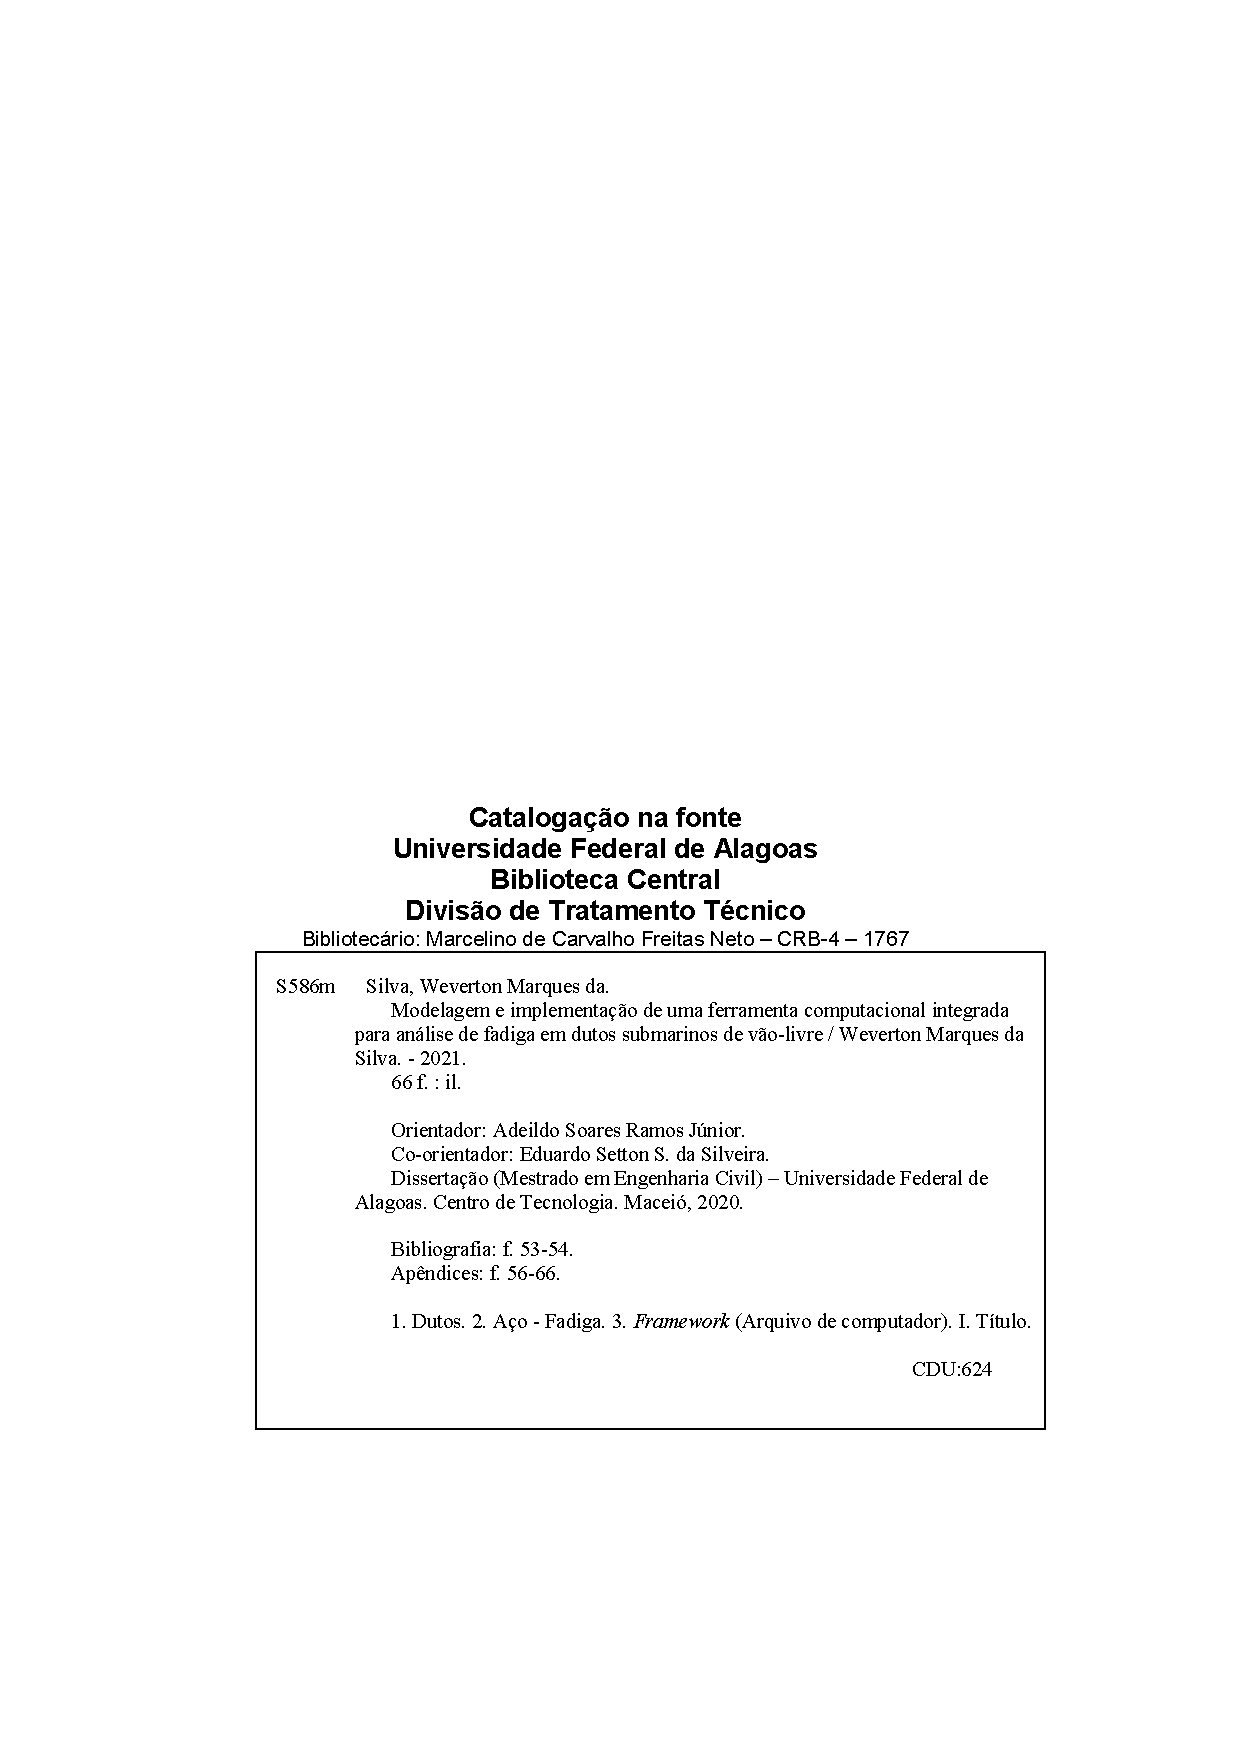
\includepdf{pretextual/ficha_catalografica.pdf}

% Inserir Folha de Aprovação
%% ---
% Assinaturas
% ---
% Isto é um exemplo de Folha de aprovação, elemento obrigatório da NBR
% 14724/2011 (seção 4.2.1.3). Você pode utilizar este modelo até a aprovação
% do trabalho. Após isso, substitua todo o conteúdo deste arquivo por uma
% imagem da página assinada pela banca com o comando abaixo:
%
% \includepdf{folhadeaprovacao_final.pdf}
%
\begin{folhadeaprovacao}
	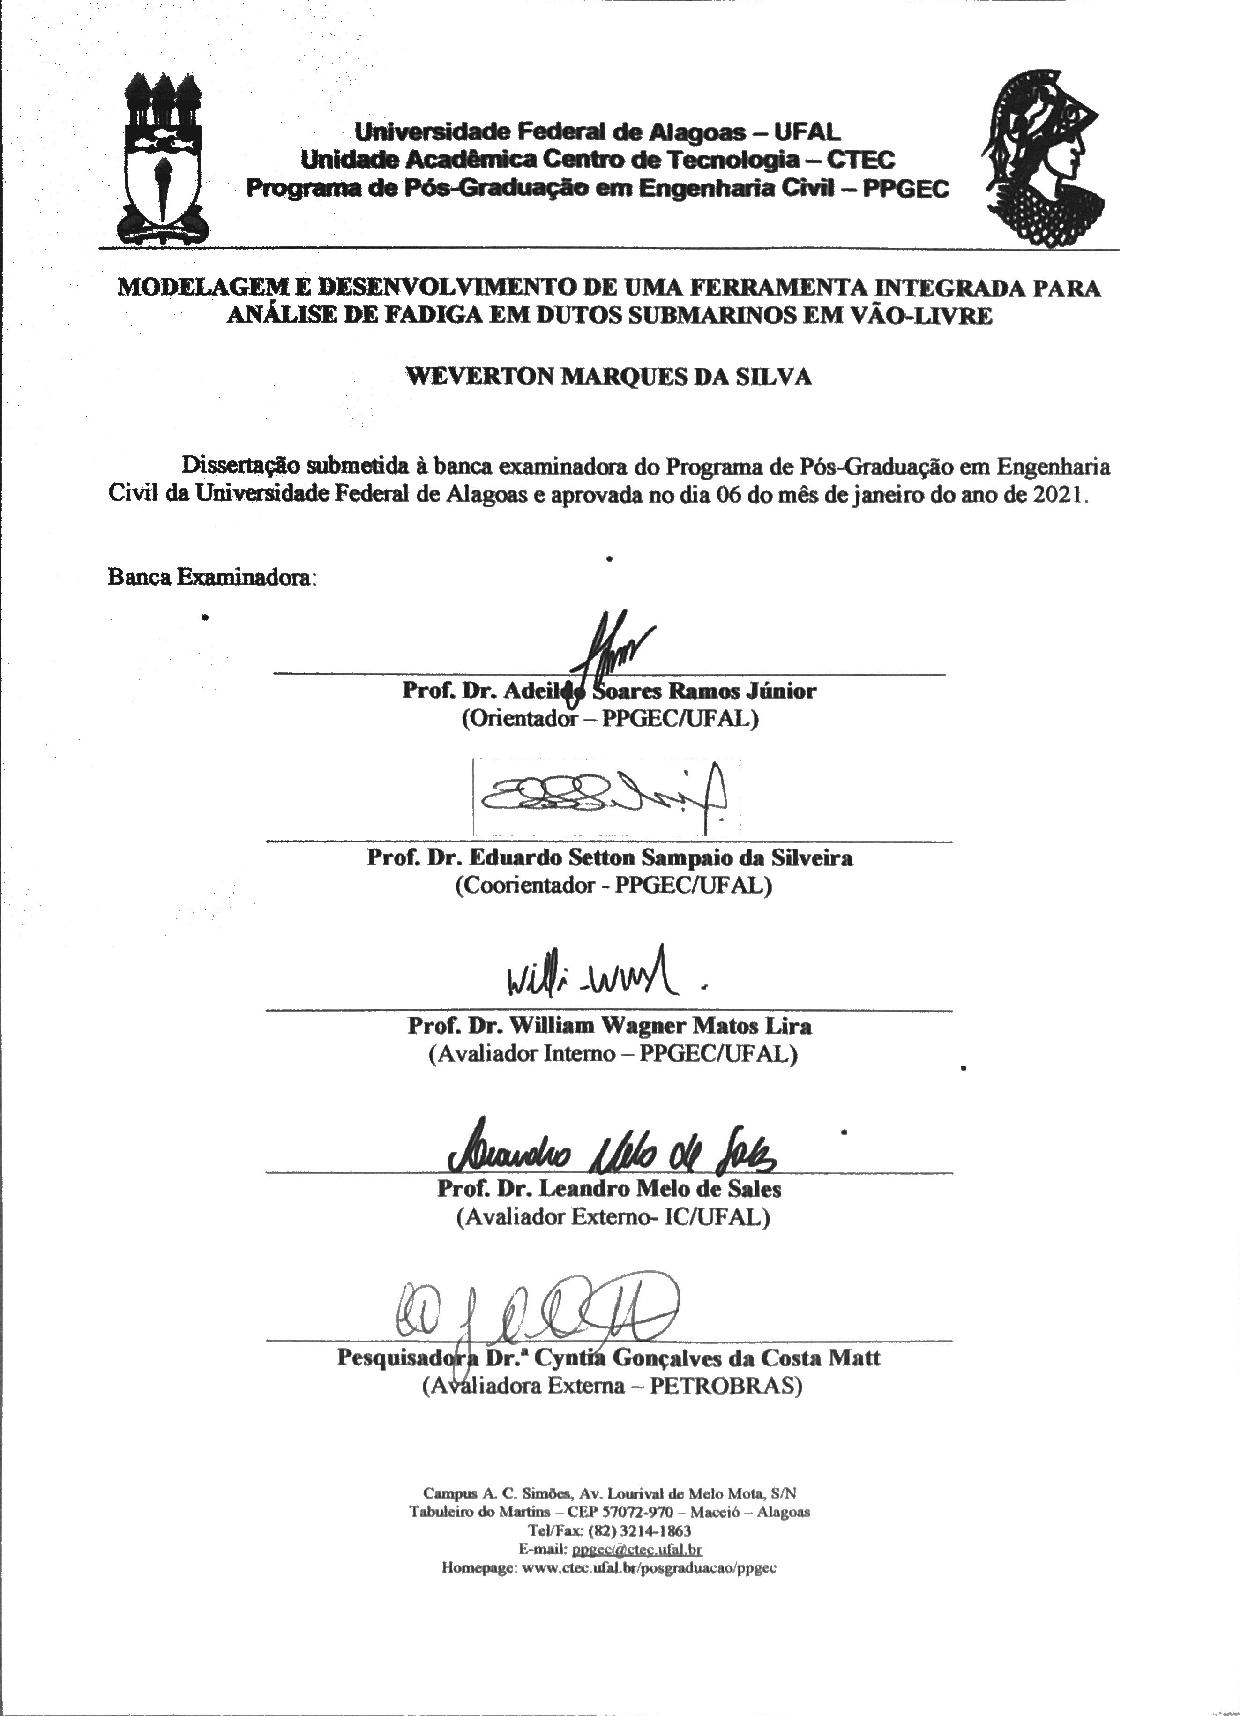
\includepdf{pretextual/folha_de_aprovacao}
	% \begin{center}
	% 	\textbf{Folha de Aprovação}
	% 	\vfill

	% 	AUTOR: \MakeUppercase{\imprimirautor}

	% 	\vfill
	% 	\imprimirtitulo
	% 	\vfill

	% 	\hspace{.45\textwidth}
	% 	\begin{minipage}{.5\textwidth}
	% 		\imprimirpreambulo
	% 	\end{minipage}%
	% 	\vfill

	% 	Trabalho aprovado. \imprimirlocal, 28 de setembro de 2016:
	% \end{center}

	% \assinatura{\textbf{\imprimirorientador} \\ Orientador}
	% \assinatura{\textbf{\imprimircoorientador} \\ Co-Orientador}
	% \assinatura{\textbf{William Wagner Matos Lira} \\ Convidado 1}
	% \assinatura{\textbf{Leandro Melo de Sales} \\ Convidado 2}

\end{folhadeaprovacao}

% Dedicatória
%% ---
% Dedicatória
% ---
\begin{dedicatoria}
   \vspace*{\fill}
   \centering
   \noindent
   \textit{ Aos meus pais XXXXXXXX e YYYYYYY, \\ por sempre estarem comigo em todos os momentos.} \vspace*{\fill}
\end{dedicatoria}
% ---

% Agradecimentos
%% ---
% Agradecimentos
% ---
\begin{agradecimentos}

Aos meus familiares por todo apoio. Especialmente, ao meus irmão, Wagner, e a minha noiva, Jhulia, que estiveram sempre ao meu lado e me ajudaram a encontrar a disposição para seguir em frente.

Agradeço ao meu orientador e coorientador pelos direcionamentos e por acreditaram na importância dos frutos desse trabalho.

Ao Laboratório de Computação Científica e Visualização pela minha participação no projeto IntegriSpan. Especialmente aos meus amigos Emerson, Josué, Jéssica e Renato. Sem a ajuda e parceria inestimável deles este trabalho não seria possível.

Aos professores do Programa de Pós-Graduação em Engenharia Civil que, com os conhecimentos transmitidos nas disciplinas, me ajudaram a elaborar esse trabalho.

\end{agradecimentos}
%% ---

% Epígrafe
%% ---
% Epígrafe
% ---
\begin{epigrafe}
    \vspace*{\fill}
	\begin{flushright}
		\textit{``Seja curioso. Leia muito. Experimente coisas novas.\\ Eu acho que muito do que as pessoas chamam de inteligência\\apenas se resume a curiosidade.''\\ % chktex 38
		          (Aaron Swartz)}
	\end{flushright}
\end{epigrafe}
% ---

% Resumo e Abstract
% ---
% RESUMOS
% ---

% RESUMO em português
\setlength{\absparsep}{18pt} % ajusta o espaçamento dos parágrafos do resumo
\begin{resumo}
TODO.

 \textbf{Palavras-chaves}: TODO.
\end{resumo}

% ABSTRACT in english
\begin{resumo}[Abstract]
 \begin{otherlanguage*}{english}
   TODO.

   \vspace{\onelineskip}
 
   \noindent 
   \textbf{Keywords}: TODO.
 \end{otherlanguage*}
\end{resumo}

% Lista de ilustrações
\pdfbookmark[0]{\listfigurename}{lof}
\listoffigures*
\cleardoublepage

% Lista de tabelas
\pdfbookmark[0]{\listtablename}{lot}
\listoftables*
\cleardoublepage

% Lista de abreviaturas e siglas
%\begin{siglas}
%  \item[ABNT] Associação Brasileira de Normas Técnicas
%  \item[abnTeX] Absurdas Normas para TeX
%\end{siglas}

% Lista de símbolos
%\begin{simbolos}
%  \item[$ \Gamma $] Letra grega Gama
%  \item[$ \Lambda $] Lambda
%  \item[$ \zeta $] Letra grega minúscula zeta
%  \item[$ \in $] Pertence
%\end{simbolos}

% Inserir o SUMÁRIO
\pdfbookmark[0]{\contentsname}{toc}
\tableofcontents*
\cleardoublepage

% ----------------------------------------------------------
% ELEMENTOS TEXTUAIS (Capítulos)
% ----------------------------------------------------------
\textual

% Ajusta o header para conter apenas o número da página
\pagestyle{simple}

% ----------------------------------------------------------
% TEXTO DA DISSERTAÇÃO
% ----------------------------------------------------------
\chapter{Modelagem numérica de dutos submarinos}
\label{chap:assentamento}


O assentamento de dutos submarinos tem sido o núcleo da engenharia \textit{offshore} por meio século.
Vários métodos e técnicas tem sido desenvolvidas e usadas para dutos submarinos~\cite{Ivic2016}.
O processo de lançamento de dutos é uma das tarefas mais desafiadoras, mesmo quando a rota ideal já está definida.
Modelar a instalação de dutos em um \textit{software} de elementos finitos para uso geral pode ser um trabalho demorado e tedioso, principalmente devido a grandes quantidades de dados da batimetria.
Na maioria das vezes, são necessárias técnicas avançadas de \textit{script} para definir o perfil do leito marinho, selecionar a rota ideal do duto e simular o processo de assentamento~\cite{VandenAbeele2013}.

A simulação do duto projetado em um ambiente tridimensional realista obtido por medições da topografia do fundo marinho, permite que os engenheiros explorem quaisquer oportunidades que o comportamento do mesmo pode oferecer para desenvolver soluções seguras e econômicas.
Por exemplo, o projetista pode analisar primeiro o comportamento do duto na batimetria original.
Se alguns dos casos de carga resultam em tensões além do limite aceitável, pode-se simular uma modificação do fundo do mar no modelo de elementos finitos.
A análise é então executada novamente para confirmar que as modificações levaram à diminuição desejada de tensão ou deformação.

O modelo de elementos finitos pode ser uma ferramenta para analisar o comportamento \textit{in-situ} de um duto.
Por comportamento \textit{in-situ} duto entenda-se a resposta do mesmo as cargas ao longo de parte do todo o seu histórico de carregamento~\cite{Bai2014}, isso pode consistir em vários casos de carga em sequência, por exemplo:

\begin{enumerate}
    \item instalação;
    \item testes de pressão (enchimento de água e do teste hidrostático);
    \item operação (enchimento com conteúdo, pressão de projeto e temperatura);
    \item ciclos de carga/descarga;
    \item flambagem lateral e vertical (\textit{upheaval});
    \item onda dinâmica e/ou de corrente;
    \item cargas de impacto.
\end{enumerate}

\citeonline{Bai2014} apresentada o processo de de análise do comportamento \textit{in-loco} desses duto com MEF, que será detalhado a seguir.


\section{Análise estática}


A modelagem da instalação do duto é o primeiro passo para o estudo do comportamento \textit{in-situ} do duto, e visa reproduzir a configuração indeformada do duto assim que lançado sobre a leito marinho.
Esta configuração serve como ponto de partida para as etapas posteriores da análise.
Mais importante do que investigar o comportamento do duto durante a instalação é garantir que a correta representação da tração e ângulo de lançamento de tal modo que consigam gerar forças residuais no duto, oriundas do atrito quando o duto se assenta sobre a batimetria.

\begin{figure}[th!]
    \centering
    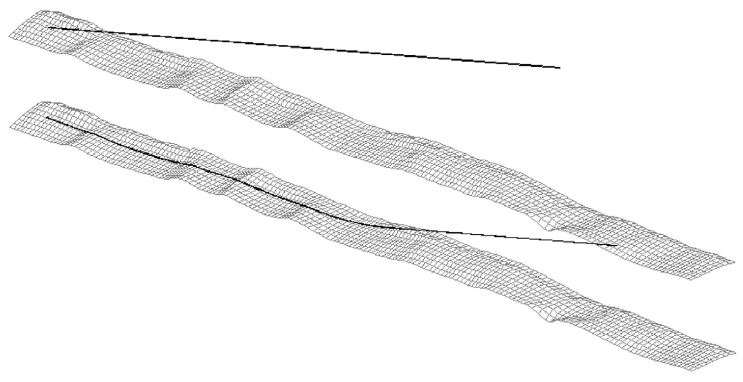
\includegraphics[width=0.7\linewidth]{imagens/lancamento_do_duto}
    \caption[]{Modelo de elementos finitos durante o lançamento.\\Fonte:~\cite{Bai2014}}\label{fig:lancamentododuto}
\end{figure}

Por simplicidade, neste trabalho, será assumido que o ângulo entre o duto e a horizontal o será nulo, isto é, o duto estará num plano horizontal que desce em direção a superfície batimétrica.
Desso modo, o modelo permitirá especificar somente a tração de lançamento.
Essa modelagem visa garantir a correta representação do contato entre o duto e a batimetria (forças de contato e ponto onde o duto toca o solo).
A Figura~\ref{fig:lancamentododuto} mostra o duto antes e durante o processo de instalação.

A medida que o duto se assenta é necessário garantir um equilíbrio estável entre o duto e o solo, o que é feito mediante um modelo representativo dessa iteração, no qual deve-se definir o atrito e rigidez do leito marinho.
No \abaqus~\cite{Dassault2018}, pode-ser relacionar a penetração e a pressão de resposta do solo por meio de uma curva de rigidez axial, além de usar modelo anisotrópico para o atrito do solo para representar as diferenças entre os atritos nas direções longitudinal e transversal.

Após a descida do duto, tem-se os processos de alagamento e desalagamento, que acarreta em mudanças no peso submerso do duto e, consequentemente, altera na sua configuração.
Esses processos podem ser facilmente modelados por uma variação numa carga vertical atuando no duto.
Mas, um duto sujeito a essa variação de carga na condição alagada sofrem grandes deformações axiais devido à mudança em geometria, e assim o duto se deforma e afunda nos vãos livres ao longo da rota do duto, como mostra a \autoref{fig:duto_alagado}.

\begin{figure}[th!]
    \centering
    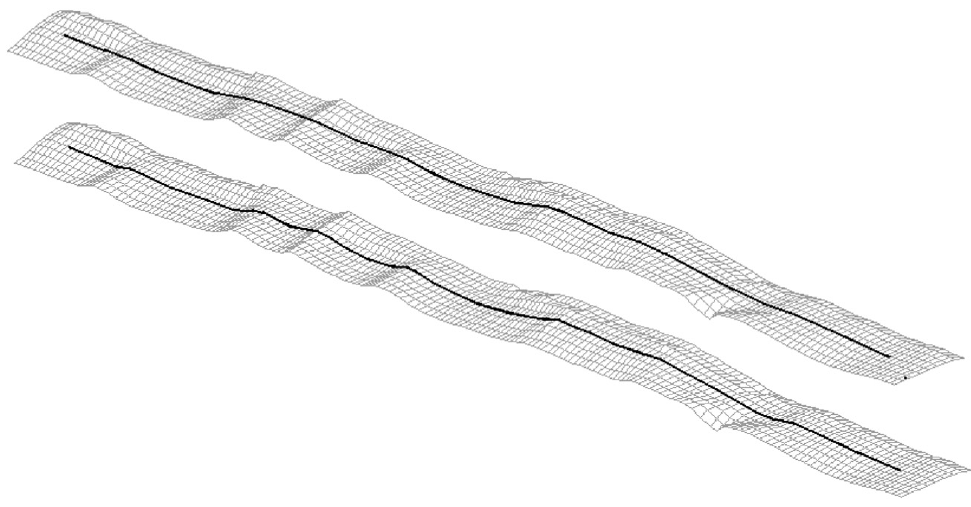
\includegraphics[width=0.7\linewidth]{imagens/duto_alagado}
    \caption[]{Modelo com o duto vazio (acima) e alagado (abaixo).\\Fonte:~\cite{Ose1999}}\label{fig:duto_alagado}
\end{figure}

Dessa maneira, é desejável que o modelo a ser estabelecido use um procedimento de análise que considere grandes deslocamentos e o efeito de alterações na área da seção do duto devido a alta tensão axial.
Além disso, é interessante qu eo modelo de material seja capaz de representar o comportamento plástico da seção do duto. No trabalho aqui proposto, não serão contempladas nas análises envolvendo efeitos de carregamentos de temperatura.

A pressão hidrostática externa é um fator importante para a capacidade de resistência de duto em águas profundas.
Como o modelo pode incluir uma estrutura tridimensional no fundo do mar, a pressão externa pode ser uma função da profundidade da água.
Já a pressão interna pode ser assumida como constante, mas a possibilidade de representar o efeito estática do conteúdo na extremidade pode ser incluído.


\section{Procedimentos e etapas de carregamento na análise de elementos finitos}


Um conceito base no \abaqus~é a divisão do histórico do cargamentos em etapas de carga. Para cada etapa, o usuário escolhe um método de análise.
Dessa forma, é possível representar qualquer sequência  e tipo de histórico de carregamento.
Por exemplo, em um passo estático, o duto pode ser carregado com gás, no passo estático seguinte descarregado, e na terceira etapa, pode-se realizar uma análise exclusiva do duto vazio.
Um histórico de carga de um modelo construído para análise é apresentado na~\autoref{tab:load_steps}.


\begin{table}[!ht]
\renewcommand{\arraystretch}{1.2}
\small
\centering
\caption[]{Histórico de carga típico em uma análise de dutos no ABAQUS.}
\label{tab:load_steps}
\begin{tabular}{cll}
\toprule[1.5pt]

\textbf{Passo} & \textbf{Ação} & \textbf{Análise} \\
\midrule
1 & Aplicação de peso próprio e empuxo do duto & Estática \\
2 & Aplicação de pressão externa hidrostática & Estática \\
3 & Aplicação de tensão leiga & Estática \\
4 & Assentamento do duto no fundo do mar (ver \autoref{fig:lancamentododuto}) & Estática \\
5 & Remoção dos elementos de guincho & Estática \\
6 & Modificando condições de contorno para a condição de instalação & Estática \\
7 & Enchimento de água para condições alagadas (ver \autoref{fig:duto_alagado}) & Estática \\
8 & Aplicação de pressão do teste hidrostático. & Estática \\
9 & Remoção da pressão do teste hidrostático & Estática \\
10 & Enchimento de gás & Estática \\
11 & Aplicação de pressão de operação & Estática \\
12 & Aplicação de temperatura de operação para a condição operacional & Estática \\
13 & Remoção de pressão e temperatura para condição de recarga & Estática \\
14 & Aplicação de carga de onda e corrente & Dinâmica \\

\bottomrule[1.25pt]
\end{tabular}
\\[6pt]
Fonte: \citeonline{Bai2014}
\end{table}

É válido de nota que a análise estática disponível no ABAQUS usada no modelo lida com respostas não lineares de efeitos de grandes deslocamentos, não-linearidade do material e não-linearidades de contorno, como contato, deslizamento e atrito (interação solo-duto). O ABAQUS usa o método de Newton para resolver as equações de equilíbrio não lineares. Portanto, a solução é obtida como uma série de incrementos com iterações para obter equilíbrio dentro de cada incremento \cite{SIMULIA2018}.

\section{Tipos de elementos}

O Abaqus dispõe de alguns tipos de elementos a serem usados no modelo do sistema de solo-duto com elementos finitos, conforme a \autoref{fig:elements_type}:

\begin{itemize}
    \item Para modelar o fundo do mar pode-ser usar os elementos rígidos do tipo R3D4 usados, ou superfícies analíticas rígidas.
    \item Os elementos do tipo PIPE31H usados para modelar o duto.
    \item Os elementos de molas usados para representar a continuidade do duto nas extremidades.
\end{itemize}

\begin{figure}[th!]
    \centering
    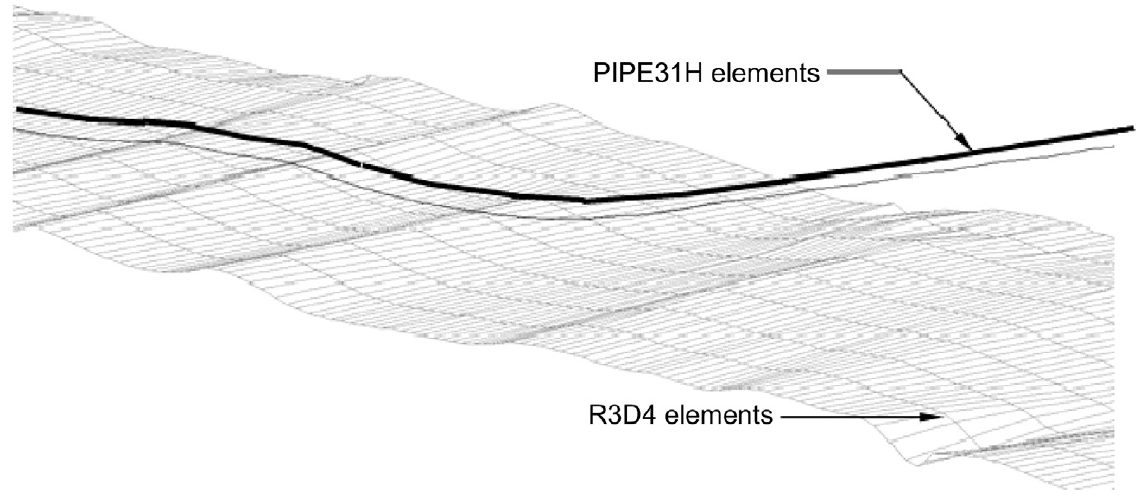
\includegraphics[width=0.8\linewidth]{imagens/elements_types}
    \caption[]{Tipos de elementos usados no modelo.\\Fonte:~\cite{Bai2014}}\label{fig:elements_type}
\end{figure}

\subsection{Elemento PIPE31/PIPE32}

A \autoref{fig:elemen_PIPE31H} mostra o elemento de duto finito 3D usado no modelo estabelecido, com 2 nós e 12 graus de liberdade.
O elemento PIPE31 usa interpolação linear, e o elemento PIPE32 interpolação quadrática.
A formulação híbrida torna o elemento adequado para casos com estruturas delgadas e problemas de contato, como um duto descendo sobre o fundo do mar.

Os elementos híbridos (PIPE31H/PIPE32H) são fornecidos para uso nos casos em que é numericamente difícil calcular as forças axiais e de cisalhamento pelo método de deslocamento próprio do Método dos Elementos Finitos.
O problema nesses casos é que pequenas diferenças em posições nodais podem causar forças muito grandes em algumas partes do modelo, o que por sua vez, causar grandes deslocamentos em outras direções.
Os elementos híbridos superam essa dificuldade usando uma formulação mais geral, na qual as forças de cisalhamento axial e transversal nos elementos são incluídas, juntamente com os deslocamentos e rotações nodais, como variáveis primárias.
Embora essa formulação torne esses elementos mais custosos computacionalmente, eles geralmente convergem muito mais rapidamente quando as rotações dos dutos são grandes.

O elemento está disponível com uma seção circular vazada de paredes finas e suporta a possibilidade de o usuário especificar pressão externa ou interna.
Elementos de paredes espessas também estão incluídos no ABAQUS.
O elemento também pode considerar alterações na área da seção do duto devido ao alto nível tensão axial do duto.

\begin{figure}[!ht]
    \centering
    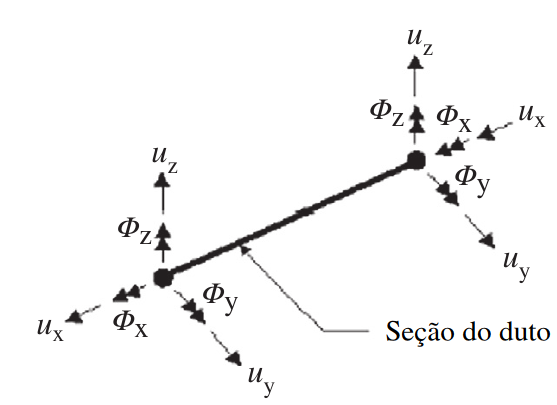
\includegraphics[width=0.5\linewidth]{imagens/elemen_PIPE31H}
    \caption[]{Elemento PIPE31.\\Fonte:~\cite{Bai2014}}\label{fig:elemen_PIPE31H}
\end{figure}

\subsection{Elemento R3D4}

O elemento rígido R3D4 de quatro nós, como mostrado na \autoref{fig:element_R3D4}, possibilita modelar superfícies complexas com geometria arbitrária e é geralmente escolhido ao modelar a topografia do fundo do mar. Uma característica muito importante do ABAQUS ao modelar o fundo do mar tem sido a possibilidade de suavizar as superfícies geradas com os elementos rígidos, o que leva a uma representação muito melhor do fundo do mar do que a superfície facetada inicial.

\begin{figure}[th!]
    \centering
    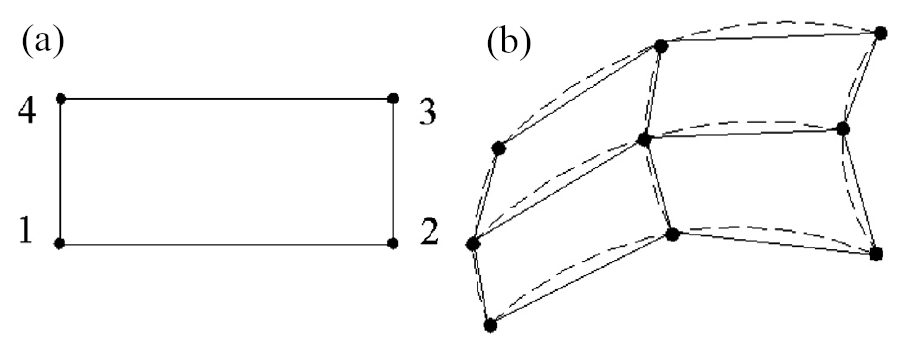
\includegraphics[width=0.7\linewidth]{imagens/element_R3D4}
    \caption[]{Elemento rígido R3D4 (a), e suavização da superfície superfície de elementos (b).\\Fonte:~\cite{Bai2014}}\label{fig:element_R3D4}
\end{figure}

A suavização é feita pela ABAQUS, criando superfícies de Bèzier com base na superfície facetada do fundo do mar formada pelos elementos rígidos. As superfícies de Bèzier resultantes, diferentemente da superfície do elemento facetado, são lisas e têm uma superfície externa com direção normal contínua. As superfícies de Bèzier não correspondem exatamente à geometria facetada da superfície rígida, mas os nós dos elementos rígidos que definem o fundo do mar permanecem sempre na superfície de Bèzier. Além disso, o usuário pode especificar o grau de suavização para controlar a geometria da superfície suavizada.

Um conjunto de elementos R3D4 que definem o fundo do mar é usado como a superfície principal chamada para aplicações de contato com os elementos do duto. Isso significa que um par de contatos (solo-duto) é definido e um modelo de interação é especificado. Esse modelo de interação geralmente consiste em uma definição de rigidez e atrito no fundo do mar.


\subsection{Superfície analítica rígida}

Outra forma deb representar a batimetria do piso marinho é utilizar uma superfície analítica rígida, isto é, uma superfície geométrica com perfis que podem ser descritos com segmentos de linha reta ou curva. Estes perfis podem ser varridos por um vetor gerador ou rotacionados em relação a um eixo para formar uma superfície tridimensional. Uma superfície analítica rígida está associada a um nó de referência de corpo rígido, cujo movimento governa toda a superfície. É importante frisar que este tipo de superfície possui apenas um lado disponível para contato, especificado de acordo com a orientação de eixos definida.

Em relação ao uso de superfícies formadas por elementos, o uso de superfícies analíticas rígidas apresenta duas vantagens:
\begin{itemize}
    \item Superfícies geométricas curvas podem ser modeladas com precisão, uma vez que é possível parametrizá-las com segmentos de linhas curvas, o que tem como resultado uma superfície mais suave, fornecendo uma melhor aproximação à restrição de contato físico.
    \item Menor custo computacional decorrente do algoritmo de contato.
\end{itemize}

Por outro lado, como desvantagens do uso deste tipo de superfície:
\begin{itemize}
    \item Uma superfície analítica rígida sempre agirá como superfície \textit{master} em uma interação de contato, impossibilitando que se modele o contato entre duas superfícies rígidas analíticas.
    \item Forças de contato e pressões não podem ser plotadas em uma superfície rígida analítica, apenas na superfície \textit{slave}.
    \item Um número muito grande de segmentos, na ordem de milhares, para definir uma superfície rígida analítica pode diminuir o desempenho. Sendo mais recomendável o uso de superfícies baseadas em elementos.
\end{itemize}


Para os casos estudados, utilizou-se uma superfície cilíndrica rígida tridimensional, conforme Figura~\ref{fig:superficie_analitica}. Para criação desta superfície é necessário fixar os pontos que definem um sistema de coordenadas locais, \textbf{a}, \textbf{b} e \textbf{c}. As coordenadas destes pontos, $(X_a, Y_a, Z_a)$, $(X_b, Y_b, Z_b)$ e $(X_c, Y_c, Z_c)$, são dadas em relação ao sistema de coordenas global. O ponto \textbf{a} define a origem do sistema de coordenadas local; o ponto \textbf{b} define o eixo-$x$ local e o ponto \textbf{c}, que se refere ao eixo-$z$ local negativo, define o vetor de geração.  Portanto, os segmentos que formam o perfil da superfície rígida são definidos no eixo $x$-$y$ local e a superfície rígida tridimensional, de acordo com o vetor de geração.

\begin{figure}[!ht]
    \centering
    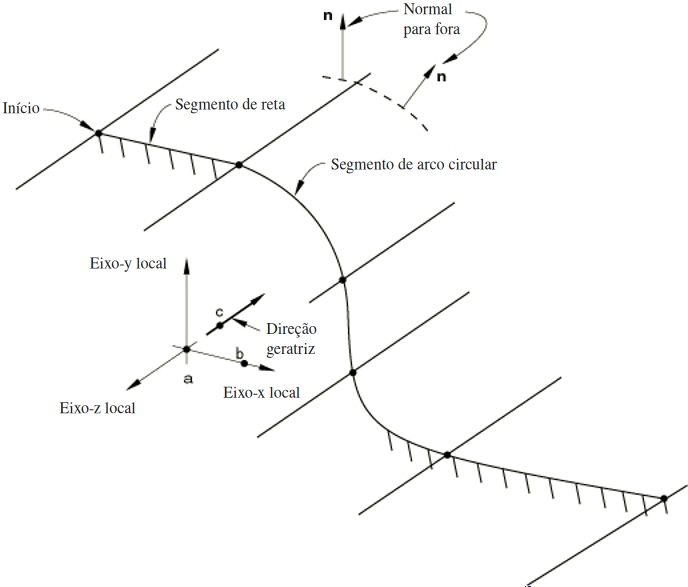
\includegraphics[width=0.7\textwidth]{imagens/superficie_analitica}
    \caption[]{\label{fig:superficie_analitica} Exemplo de superfície analítica rígida.\\Fonte: \citeonline{SIMULIA2018}}
\end{figure}

\chapter{Planejamento de experimentos}
\label{chap:doe}

% \begin{figure}[!hbt]
% 	\centering
% 	\caption{Símbolo da UFAL}
% 	\label{fig:1_possuem_celular}
% 	
\includegraphics[width=0.25\textwidth]{imagens/ufal}
% \end{figure}

Como visto anteriormente, o problema da modelagem do assentamento de dutos envolve um número considerável de variáveis, principalmente se o duto for constituído de trechos com de materiais ou o solo for 

\section{SIMULIA ISight}

Além desses recurso o ISight permite gerar facilmente um gráfico de Pareto, que é uma forma eficiente de comunicar o resultado de uma análise de DOE.

\subsection{Gráfico de Pareto}

Um gráfico de Pareto mostra os efeitos relativos dos fatores em uma resposta, conforme determinado pela análise de regressão do conjunto de dados. É um gráfico de barras ordenado que exibe os efeitos de cada fator em uma resposta selecionada, em que os fatores são listados na ordem do maior efeito para o menor efeito. Pode-se utilizar cores para as barras apara diferencias efeitos positivos e negativos. Portanto, este gráfico pode ser usado para identificar os fatores com os efeitos mais significativos, ou com maior contribuição, para as respostas.

A classificação dos efeitos apresentados no gráfico de Pareto é determinada pela ordenação dos coeficientes escalonados e normalizados de um ajuste polinomial de mínimos quadrados padrão de segunda ordem para os dados do componente. Se dados suficientes estiverem disponíveis - pelo menos $(N + 1) (N + 2) / 2$ pontos, onde $N$ é o número de entradas - e cada entrada tem pelo menos três níveis / valores distintos, um modelo polinomial de segunda ordem completo, incluindo todas as interações bidirecionais, é adequado aos dados. O número mínimo de pontos requeridos é $(N + 1)$, resultando em um ajuste polinomial linear. Se o número de pontos de dados estiver entre $(N + 1)$ e $(N + 1) (N + 2) / 2$, um polinômio de segunda ordem é construído (termos de interação quadrática, bidirecional adicionados até que nenhum grau de liberdade permaneça).

Antes de ajustar o modelo polinomial, os dados de entrada são primeiramente escalonados para variar de -1 a 1 e o ajuste de mínimos quadrados é executado nesses dados. O escalonamento é executado de forma que as contribuições possam ser comparadas de forma mais justa, porque tanto a magnitude dos fatores quanto a quantidade que eles variam afetam os dados usados na construção do modelo de superfície de resposta. Os coeficientes do modelo resultantes da regressão de mínimos quadrados aplicada aos dados escalonados são normalizados pela soma
dos coeficientes e dividindo cada coeficiente por essa soma de todos os coeficientes.

% ----------------------------------------------------------
% ELEMENTOS PÓS-TEXTUAIS (Referências, Glossário, Apêndices)
% ----------------------------------------------------------
\postextual

\bibliography{bibliografia}

\end{document}
